\chapter{Comparision of free IDSs}
\minitoc
\emph{This chapter will cover a comparision of three freely available Intrusion Detection Systems. Two signature-based Network Intrusion Detection Systems and one anomaly-based Network Intrusion Detection System. }

\section{Network Intrusion Detection Systems}

Since my interest is concentrated on computer networks, only \textbf{Network} IDSs will be listed and compared. NIDSs differ of HIDSs in the fact a NIDS protects an entire network, whereas a HIDS only protect a single host.

\section{The tools}

Below is is overview of the tools that will be compared, with a brief describtion about them.
\begin{itemize}
\item \textbf{Snort:} Snort is a lightweight signature-based Network Intrusion Detection (and Prevention) system written by Martin Roesch in 1999 and is written in C and C++. It is lightweight in a way that the sourcecode is about 100KB in size and that it takes only a few minutes to compile. With the use of the ruleset, Snort is capable to detect stealth port scans, buffer overflows, SMB probes, DOS attacks and much more kinds of attacks \citep{SnortChap3}. In addition, Snort is highly extendable \citep{SnortSF}.
\item \textbf{Suricata:} Suricata is another example of a signature-based Network Intrusion Detection (and Preventing) System written in C and developed by the Open Information Security Foundation (OISF) \citep{Suricata2}. It claims to be a next generation NIDS that will bring new technologies and ideas to the domain of intrusion detection \citep{Suricata1}. One could see it as the competitor of Snort.
\item \textbf{Bro:} Bro is an anomaly-based Network Intrusion Detection developed by Vern Paxson in 1999 and is written in C++ \citep{Bro1}. In contrast to Snort and Suricata, Bro offers much more functionality than only packet sniffing, logging and alerting. With the scripting language (Python or Perl) provided by Bro, one can extend Bro's functionality to its own needs \citep{Bro2}.
\end{itemize}

\section{Comparision}

Below is a table that compares the features of Snort, Suricata and Bro, based on a literature study \citep{Comp1, Comp2, Comp3}

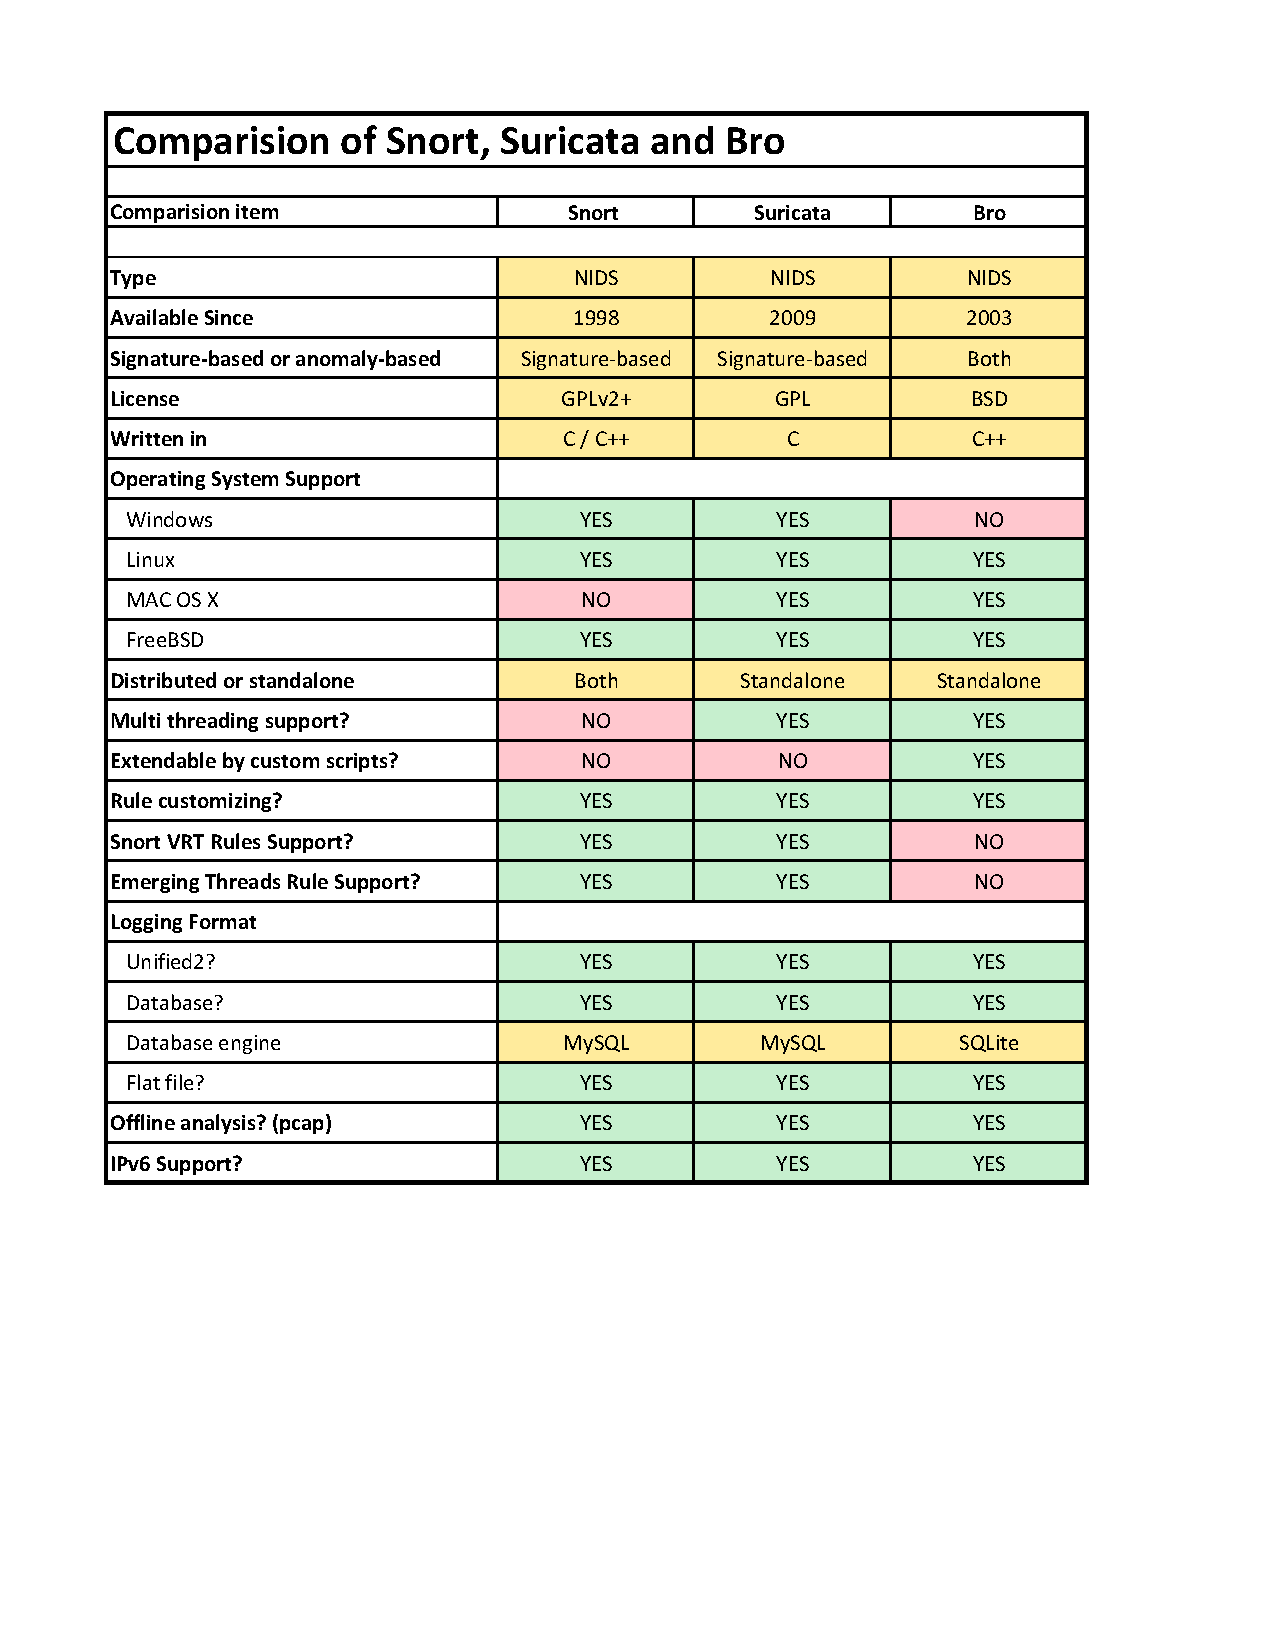
\includepdf{Comparision.pdf}

Since Snort is praised for its functionality and used by many people, I decided to test whether Snort is really as good as is stated. Therefore, Snort is picked as the tool that will be tested.